%!TEX root =  ./JanasJanssenCuffaro-August2019.tex
%SECTION 4
%\section{Correlation arrays, polytopes and the CHSH inequality} \label{3}
%Four settings and two outcomes per setting
%From three to four different settings:
%A Setup with four settings and two outcomes per setting: the CHSH inequality

In the preceding sections we studied the Mermin setup, which involves two parties and three settings per party. In Section \ref{1}, we analyzed the case with two outcomes per setting; in Section \ref{2}, we extended our analysis to three and more outcomes per setting. In this section, we return to the simple case of two outcomes per setting. However, the two parties now get to choose from two different pairs of settings, rather than from the same triplet of settings. In other words, we replace the Mermin setup by the more common setup for which the CHSH inequality \citep{CHSH} was formulated and tested. As in Section \ref{1}, we focus on correlations found in measurements performed on a pair of spin-$\frac12$ in the singlet state and on raffles designed to simulate these correlations. 

\begin{figure}[ht]
 \centering
   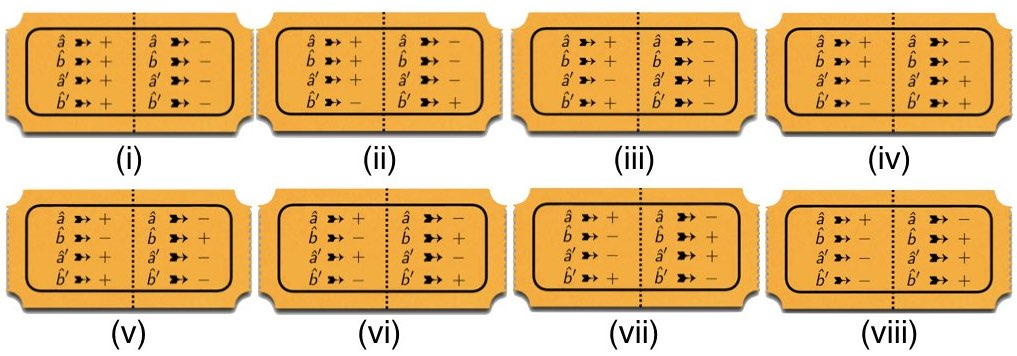
\includegraphics[width=4.5in]{raffle-tickets-4set2out-i-thru-viii.jpeg} 
   \caption{Raffle tickets for four settings and two outcomes.}
   \label{raffle-tickets-4set2out-i-thru-viii}
\end{figure}

Our goal in this section is to recover the CHSH inequality and the corresponding Tsirelson bound  in the Bub-Pitowsky-inspired framework developed in Sections \ref{1}--\ref{2}. The key to achieving this objective is to note that the CHSH setup, in which Alice and Bob pick from two \emph{different pairs} of settings, $(\hat{a}, \hat{b})$ and $(\hat{a}', \hat{b}')$, can be treated as a special case of a straightforward generalization of the Mermin setup in which they pick from the \emph{ same quartet} of settings $(\hat{a}, \hat{b}, \hat{a}', \hat{b}')$. The special case of this generalized Mermin setup is that Alice never actually uses the settings $(\hat{a}', \hat{b}')$ and that Bob never actually uses the settings  $(\hat{a}, \hat{b})$. Nothing prevents us, however, from adding cells for the unused combinations of settings to the correlation arrays for the CHSH setup. In this way, the $2 \times 2$ correlation arrays for the CHSH setup turn into $4 \times 4$ correlation arrays (see, e.g., Figure \ref{CA-4set2out-raffle-viii}) that are similar to the $3 \times 3$ ones for the Mermin setup (see, e.g.,  Figures \ref{CA-3set2out-Mermin}, \ref{CA-3set2out-raffles-i-thru-iv} and \ref{CA-3set2out-raffle-mix}). The off-diagonal cells of these $4 \times 4$ correlation arrays can be parametrized by six anti-correlation coefficients, two of which ($\chi_{ab}$ and $\chi_{a'b'}$) do not play a role in the CHSH setup. The CHSH inequality and the Tsirelson bound in this case are conditions on the remaining four, $\chi_{aa'}$, $\chi_{ab'}$, $\chi_{ba'}$ and $\chi_{bb'}$. To derive the CSHS inequality, we use the kind of raffles we introduced in Section \ref{1.4}. As in Section \ref{1.5}, we derive the corresponding Tsirelson bound from the positive semi-definiteness of the anti-correlation matrix $\chi$, which in this case is a symmetric $4 \times 4$ matrix with $1$'s on the diagonal and the six anti-correlation coefficients as its off-diagonal elements. 

\begin{figure}[ht]
 \centering
   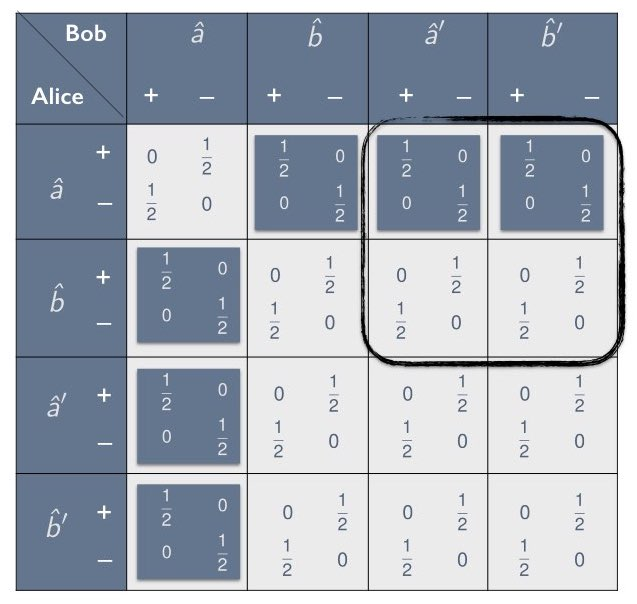
\includegraphics[width=3.5in]{CA-4set2out-raffle-viii.jpeg} 
   \caption{Correlation array for a raffle with a basket of tickets of type (viii) (see Figure \ref{raffle-tickets-4set2out-i-thru-viii}). Blue-on-white cells show perfect anti-correlation; white-on-blue cells show perfect correlation. The four cells in the upper-right corner are the ones actually probed in tests of the CHSH inequality.}
   \label{CA-4set2out-raffle-viii}
\end{figure}

Figure \ref{raffle-tickets-4set2out-i-thru-viii} shows the eight different types of raffle tickets for the CHSH setup. Figure \ref{CA-4set2out-raffle-viii} shows the correlation array for a raffle with a basket containing only type-(viii) tickets. Six of the off-diagonal cells in this correlation array show a perfect correlation, the other six show a perfect anti-correlation. This means that the values of the six anti-correlation coefficients parametrizing these twelve cells are:
\begin{equation}
\chi_{ab}^{\mathrm{(viii)}} = \chi_{aa'}^{\mathrm{(viii)}} = \chi_{ab'}^{\mathrm{(viii)}} = -1, \quad \chi_{ba'}^{\mathrm{(viii)}} = \chi_{bb'}^{\mathrm{(viii)}} = \chi_{a'b'}^{\mathrm{(viii)}} = 1.
\label{chi values for ticket (viii)}
\end{equation}
These values can also be read directly off ticket (viii).  

 \begin{table}[ht]
\centering
\begin{tabular}{|c||c|c|c|c||c|}
\hline
ticket & \quad $\chi_{aa'}^{\mathrm{(k)}}$ \quad & \quad $\chi_{ab'}^{\mathrm{(k)}}$ \quad & \quad $\chi_{ba'}^{\mathrm{(k)}}$ \quad & \quad $\chi_{bb'}^{\mathrm{(k)}}$ \quad &  $\chi_{aa'}^{\mathrm{(k)}} +\chi_{ab'}^{\mathrm{(k)}}$ \quad \\[.1cm] 
 &  &  &  &  &  \quad $+\chi_{ba'}^{\mathrm{(k)}} - \chi_{bb'}^{\mathrm{(k)}}$ \quad \\[.1cm]
\hline
 (i) & $+1$ & $+1$ & $+1$ & $+1$ & $2$ \\[.1cm]
 (ii) & $+1$ & $-1$ & $+1$ & $-1$ & $2$ \\[.1cm]
 (iii) & $-1$ & $+1$ & $-1$ & $+1$ & $-2$ \\[.1cm]
(iv) & $-1$ & $-1$ & $-1$ & $-1$ & $-2$ \\[.1cm]
 (v) & $+1$ & $+1$ & $-1$ & $-1$ & $2$ \\[.1cm]
 (vi) & $+1$ & $-1$ & $-1$ & $+1$ & $-2$ \\[.1cm]
 (vii) & $-1$ & $+1$ & $+1$ & $-1$ & $2$ \\[.1cm]
(viii) & $-1$ & $-1$ & $+1$ & $+1$ & $-2$ \\[.1cm]
 \hline
\end{tabular}
\caption{Values of four of the anti-correlation coefficients for tickets (i)--(viii) in Figure \ref{raffle-tickets-4set2out-i-thru-viii}. The final column shows the values for a linear combination of these coefficients.}
\label{values of chi-4set2out}
\end{table}
%$\ ($\mathrm{k = i \ldots viii}$), 

In the CHSH setup, data are taken only for the four combinations of settings corresponding to the four cells in the upper-right corner of these $4 \times 4$ correlation arrays. These cells are characterized by four of the six anti-correlation coefficients in Eq.\ (\ref{chi values for ticket (viii)}). Table \ref{values of chi-4set2out} lists their values for all eight tickets in Figure \ref{raffle-tickets-4set2out-i-thru-viii}. The final column gives the value for a linear combination of these four anti-correlation coefficients. Note that for tickets (i), (ii), (v) and (vii), this quantity is equal to 2, while for tickets (iii), (iv), (vi) and (viii), it is equal to $-2$. For a raffle with any mix of tickets of type (i) through (viii), this quantity must therefore lie between $-2$ and $2$:
%(cf.\ Section \ref{1.4}, note \ref{checking averaging of chi}):
\begin{equation}
-2 \le \chi_{aa'} + \chi_{ab'} + \chi_{ba'} - \chi_{bb'} \le 2.
\label{CHSH inequality}
\end{equation}
This is the CHSH inequality \citep[p.\ 68]{Bub 2016}.

We now want to connect the raffles with tickets for the present case of four settings to the raffles in Section \ref{1.4} for the case of three settings. An obvious way to do this is to ignore one of the four settings and have Alice and Bob choose between the remaining three. In that case, there are only three anti-correlation coefficients, which will satisfy the inequality in Eq.\ (\ref{Mermin inequality CHSH-like}) for the Mermin setup. One could object, however, that this way of recovering Eq.\ (\ref{Mermin inequality CHSH-like}) requires that we consider results found for combinations of settings Alice and Bob are not actually using in the CHSH setup. To avoid this objection, suppose Bob's setting $\hat{b}'$ is the same as Alice's setting $\hat{b}$. This means that we restrict ourselves to tickets with the same values for $\hat{b}$ and $\hat{b}'$. These are the tickets (i), (iii), (vi) and (viii) in Figure \ref{raffle-tickets-4set2out-i-thru-viii}. Focusing on the rows for those four tickets in Table \ref{values of chi-4set2out} and using that, in those rows, $\chi_{bb'} = 1$ and $\chi_{ab'} = \chi_{ab}$, we see that the inequality in Eq.\ (\ref{CHSH inequality}) reduces to:
\begin{equation}
-1 \le \chi_{aa'} + \chi_{ab} + \chi_{ba'} \le 3.
\label{CHSH2Bell}
\end{equation}
If $\hat{a}'$ is relabeled $\hat{c}$, this inequality turns into the one in Eq.\ (\ref{Mermin inequality CHSH-like}) for the Mermin setup. Note that this is the form in which \citet{Bell 1964} originally derived the Bell inequality (see Section \ref{1.1}).

As was stressed in Section\ \ref{1.4} for the case of three settings, however, the CHSH inequality is a necessary but not sufficient condition for classical correlations. To obtain a complete characterization of the correlations allowed classically, we once again examine their geometrical representation.

The tickets in Table \ref{values of chi-4set2out} give the coordinates of eight points in the four-dimensional space of anti-correlation coefficients $\chi_{aa'},\chi_{ab'},\chi_{ba'},\chi_{bb'}$. Since the anti-correlation coefficients of a classical mixed state will be a weighted average of those for the classical pure states, we may interpret those eight points as vertices of some convex hull. This is the local polytope, i.e., the set of of anti-correlation coefficients $\chi_{aa'},\chi_{ab'},\chi_{ba'},\chi_{bb'}$ that can be simulated by such raffles.

While we cannot visualize this four--dimensional polytope, some geometric observations can be made. The eight vertices may be viewed as four pairs of antipodal points, with the four line segments between the pairs being mutually orthogonal. As was noted by \citet[p. 5]{Pitowsky 2008}, this polytope is the 4-dimensional octahedron or hyperoctahedron \citep[p.\ 112]{Bub 2016}. It has a total of 16 facets, half of which are given by the inequalities
\begin{eqnarray}
-2 \le \;\, \chi_{aa'} + \chi_{ab'} + \chi_{ba'} - \chi_{bb'} \; \le 2, & & \label{CHSH-ineq 1} \\[.2cm]
-2\le -\chi_{aa'}+\chi_{ab'}-\chi_{ba'}-\chi_{bb'} \; \le  2,  & & \label{CHSH-ineq 2}  \\[.2cm]
-2\le \;\, \chi_{aa'}-\chi_{ab'}-\chi_{ba'}-\chi_{bb'} \; \le  2, & & \label{CHSH-ineq 3}  \\[.2cm]
-2\le  -\chi_{aa'}-\chi_{ab'}+\chi_{ba'}-\chi_{bb'} \; \le  2. & & \label{CHSH-ineq 4}
\end{eqnarray}
Eq.\ (\ref{CHSH-ineq 1}) is just the CHSH inequality stated above when Alice and Bob use settings $(\hat{a},\hat{b})$ and $(\hat{a}',\hat{b}')$, respectively. We may obtain the others similarly by reversing some of the settings. For instance, Eq.\ (\ref{CHSH-ineq 2}) is the CHSH inequality if Bob were to use setting $-\hat{b}$ instead of $\hat{b}$. For our purposes, we will regard each of them as a CHSH inequality.

For the remaining eight facets, note that all coordinates of the eight vertices are $\pm 1$, with $+1$ occurring an even number of times. Hence these are eight of the sixteen vertices for a four-dimensional hypercube, which is the non-signaling polytope in the CHSH setup. It bounds the local polytope, thus providing the remaining eight facets which \citet[p.\ 3, Eq.\ (2)]{Pitowsky 2008} refers to as ``trivial'':
\begin{equation}
-1\leq \chi_{aa'}\leq 1,\quad -1\leq \chi_{ba'}\leq 1,\quad -1\leq \chi_{ab'}\leq 1,\quad -1\leq \chi_{bb'}\leq 1.
\end{equation}
In the case of the Mermin example, the four facets of the classical tetrahedron already sufficed to restrict the correlations to the non-signaling cube. This is not sufficient in the present setup. For instance, the values $\chi_{aa'}=2,\chi_{ab'}=\chi_{ba'}=\chi_{bb'}=0$ are allowed by the CHSH inequalities but lie outside the non-signaling hypercube. It is thus necessary to include the hypercube facets explicitly.

The parts of the local polytope which lie on one of these hypercube facets are particularly notable. If we restrict our attention to the facet $\chi_{bb'}=1$, for instance, then we are looking at what part of the local polytope falls in the region parametrized by $\chi_{aa'}$, $\chi_{ab'}$ and $\chi_{ba'}$. Since each of these coefficients has magnitude 1, we are working with a copy of the non-signaling cube for three outcomes. The inequalities in Eqs. (\ref{CHSH-ineq 1})--(\ref{CHSH-ineq 4})) then simplify to
\begin{eqnarray}
-1 \le \;\, \chi_{aa'} + \chi_{ab'} + \chi_{ba'}\; \le 3, & & \\[.2cm]
-1\le -\chi_{aa'}+\chi_{ab'}-\chi_{ba'} \; \le  3, & & \\[.2cm]
-1\le \;\, \chi_{aa'}-\chi_{ab'}-\chi_{ba'} \; \le  3, & & \\[.2cm]
-1\le  -\chi_{aa'}-\chi_{ab'}+\chi_{ba'} \; \le 3. & &
\end{eqnarray}
Aside from having $\hat{a}',\hat{b}'$ instead of $\hat{c},\hat{b}$, this system of inequalities is identical to those that generated the classical tetrahedron in the Mermin setup (see Eqs.\ (\ref{Mermin inequality CHSH-like (i)})--(\ref{Mermin inequality CHSH-like (iv)})). Hence the local polytope in the CHSH setup contains a copy of the classical tetrahedron, occurring on the $\chi_{bb'}=1$ facet of the non-signaling hypercube; this facet is itself a copy of the non-signaling cube.
%(This is actually true in general: The sixteen cells of the 4-dimensional octahedron are regular tetrahedra, as may be shown by considering the case where the CHSH inequality reaches its maximum value.) 

We now consider the analogous quantum story, i.e., the correlations of the singlet state for the CHSH setup. Cells in the correlation array for the CHSH setup are no different from cells in the correlation array for the Mermin setup given in Section \ref{1.5}. The anti-correlation coefficients for any combination of measurement directions $\vec{e}_a$ and $\vec{e}_b$ are given by  
\begin{equation}
\chi_{ab} =-\langle \hat{S}_{1a}\hat{S}_{2b}\rangle_{00} =  \cos\varphi_{ab}
\end{equation}
(see Eq.\ (\ref{chi2angle}) with the standard deviations $\sigma_{1a}$ and $\sigma_{2b}$ set equal to 1). 

We now introduce the anti-correlation matrix
\begin{equation}
\chi=
\begin{pmatrix}
\chi_{aa} & \chi_{ab} & \chi_{aa'} & \chi_{ab'} \\[.2cm]
\chi_{ba} & \chi_{bb} & \chi_{ba'} & \chi_{bb'} \\[.2cm]
\chi_{a'a} & \chi_{a'b} & \chi_{a'a'} & \chi_{a'b'} \\[.2cm]
\chi_{b'a} & \chi_{b'b} & \chi_{b'a'} & \chi_{b'b'}.
\end{pmatrix}=
\begin{pmatrix}
1 & \cos \varphi_{ab} & \cos \varphi_{aa'} & \cos \varphi_{ab'} \\[.2cm]
\cos \varphi_{ab} & 1 & \cos \varphi_{ba'} & \cos \varphi_{bb'} \\[.2cm]
\cos \varphi_{aa'} &\cos \varphi_{ba'} & 1 & \cos \varphi_{a'b'} \\[.2cm]
\cos \varphi_{ab'} & \cos \varphi_{bb'} & \cos \varphi_{a'b'} & 1.
\end{pmatrix}.
\label{CHSH-matrix}
\end{equation}
Using that $\cos{\varphi_{ab}} = \vec{e}_a \cdot \vec{e}_b$ etc.\ and that $\vec{e}_a = (a_x, a_y, a_z)$, etc., we can factorize this matrix as (cf.\ Eqs.\ (\ref{QM10})--(\ref{QM12})):
%\begin{eqnarray}
%\chi 
%& \!\! = \!\! &
%\begin{pmatrix}
%\vec{e}_a \! \cdot  \vec{e}_a &  \vec{e}_a \! \cdot  \vec{e}_b  &   \vec{e}_a \! \cdot  \vec{e}_{a'} & \vec{e}_a \! \cdot  \vec{e}_{b'} \\
%\vec{e}_b \! \cdot  \vec{e}_a & \vec{e}_b \! \cdot  \vec{e}_b & \vec{e}_b \! \cdot  \vec{e}_{a'} & \vec{e}_b \! \cdot  \vec{e}_{b'} \\
%\vec{e}_{a'} \! \cdot  \vec{e}_a & \vec{e}_{a'} \! \cdot  \vec{e}_b & \vec{e}_{a'} \! \cdot  \vec{e}_{a'} & \vec{e}_{a'} \! \cdot  \vec{e}_{b'} \\
%\vec{e}_{b'} \! \cdot  \vec{e}_a & \vec{e}_{b'} \! \cdot  \vec{e}_b & \vec{e}_{b'} \! \cdot  \vec{e}_{a'} & \vec{e}_{b'} \! \cdot  \vec{e}_{b'}
%\end{pmatrix} \nonumber \\
%& \!\! = \!\!  &
%\begin{pmatrix}a_x & a_y & a_z \\ b_x & b_y & b_z \\ a'_x & a'_y & a'_z \\ b'_x & b'_y & b'_z \end{pmatrix}
%\begin{pmatrix} a_x & b_x & a'_x & b'_x \\ a_y & b_y & a'_y & b'_y  \\ a_z & b_z & a'_z & b'_z.  \end{pmatrix}
%\equiv T^\top T.
%\end{eqnarray}
\begin{equation}
\chi = 
\begin{pmatrix}
a_x & a_y & a_z \\[.2cm]
b_x & b_y & b_z \\[.2cm] 
a'_x & a'_y & a'_z \\[.2cm] 
b'_x & b'_y & b'_z 
\end{pmatrix}
\begin{pmatrix} 
a_x & b_x & a'_x & b'_x \\[.2cm]
a_y & b_y & a'_y & b'_y  \\[.2cm]
a_z & b_z & a'_z & b'_z.  
\end{pmatrix}
\equiv L^\top L.
\end{equation}
This factorization implies that, given any vector $\vec{v}=(v_a,v_b,v_c)^\top$, one has 
\begin{equation}
\vec{v}^\top \! \chi\vec{v} = \vec{v}^\top L^\top L \vec{v} = (L\vec{v})^\top L \vec{v} \geq 0,
\end{equation}
where in the last step we used that this quantity is the length squared of the vector $L\vec{v}$. Hence $\chi$ is positive semi-definite (cf.\ Eq.\ (\ref{inf the 4})).

The set of such $4 \times 4$ matrices---that is, those which are symmetric, have $1$'s on the diagonal and are positive semi-definite---is conventionally known as the 4-elliptope. The terminology is an obvious generalization of the elliptope for the $3 \times 3$ case and for the purposes of this section we refer to the latter as the 3-elliptope. The 4-elliptope, being parametrized by six anti-correlation coefficients, is a six-dimensional set; like the 3-elliptope, it is moreover convex (since any weighted average of two positive semi-definite matrices is itself positive semi-definite). As noted before, however, the values of $\chi_{ab}$ and $\chi_{a'b'}$ are not provided in the context of the CHSH inequality. As such we must project this convex set to the four-dimensional space of the coefficients $\chi_{a'b'}$, $\chi_{aa'}$, $\chi_{ab'}$ and $\chi_{ba'}$. The resulting four-dimensional convex set, a shadow of the 4-elliptope, represents the class of correlations that Alice and Bob can obtain by measuring the singlet state using the settings $(\hat{a}, \hat{b})$ and $(\hat{a}', \hat{b}')$, respectively.\footnote{In the present case, we can further note that the four columns of $L$ are unit vectors in three-dimensional space. As such they must be linearly dependent, which implies that zero is an eigenvalue of $L$ (and thus of $\chi$ as well). Hence $\chi$ is not positive definite and must lie in the five-dimensional boundary of the 4-elliptope. However, this restriction plays no role upon projecting to the shadow of the 4-elliptope and so will not be elaborated upon further.}

Like the local polytope, neither the 4-elliptope nor its projected shadow can be visualized in its totality, yet some geometrical conclusions can still be drawn. For instance, since these  anti-correlation coefficients are cosines, their magnitude does not exceed 1. Hence, the set of quantum correlations is contained within the non-signaling hypercube. Moreover, this set contains the local polytope. To see this, consider a configuration in which the unit vectors for all four measurement settings lie along the same line, i.e., are either parallel or anti-parallel. This configuration can be realized in eight ways. Then all the cosines are $\pm 1$, with $+1$ occurring an even number of times. This corresponds directly to the eight vertices of the local polytope (i.e., the rows of Table\ \ref{values of chi-4set2out}). Since the 4-elliptope (and therefore its shadow) is convex, we conclude that the set of quantum correlations does indeed include the local polytope.

It remains to show that the set of quantum correlations is larger than the local polytope. Recall that we can use $-\hat{S}_{2b}$ as a stand-in for $\hat{S}_{1b}$ when evaluating the expectation value $ \langle \hat{S}_{1a}\hat{S}_{1b}\rangle_{00}$ (see the end of  Section \ref{1.5}):
\begin{equation}
\chi_{ab} =-\langle \hat{S}_{1a}\hat{S}_{2b}\rangle_{00} = \langle \hat{S}_{1a}\hat{S}_{1b}\rangle_{00}.
\end{equation}
Now note that
\begin{equation}
\Big\langle \Big(\hat{S}_{1a'}-\frac{1}{\sqrt{2}}\hat{S}_{1a}-\frac{1}{\sqrt{2}}\hat{S}_{1b}\Big)^{\!2}\Big\rangle_{00}
= 2-\sqrt{2}\chi_{aa'}-\sqrt{2}\chi_{a'b}+\chi_{ab}\geq 0.
\label{CHSH-Tsirelson 1}
\end{equation}
Similarly,
\begin{equation}
\Big\langle \Big( \hat{S}_{1b'}-\frac{1}{\sqrt{2}}\hat{S}_{1a}+\frac{1}{\sqrt{2}}\hat{S}_{1b} \Big)^{\!2} \Big\rangle_{00}
= 2-\sqrt{2}\chi_{ab'}+\sqrt{2}\chi_{bb'}-\chi_{ab}\geq 0.
\label{CHSH-Tsirelson 2}
\end{equation}
Adding these two inequalities, we arrive at
\begin{equation}
2-\sqrt{2}\chi_{aa'}-\sqrt{2}\chi_{a'b} + 2-\sqrt{2}\chi_{ab'}+\sqrt{2}\chi_{bb'} \geq 0,
\label{CHSH-Tsirelson 3}
\end{equation}
which can be rewritten as
\begin{equation}
\chi_{aa'}+\chi_{a'b}+\chi_{ab'}-\chi_{bb'} \leq 2\sqrt{2}.
\label{CHSH-Tsirelson 4}
\end{equation}
This is the Tsirelson bound for the CHSH setup \citep[p.\ 68]{Bub 2016}. 

\begin{figure}[ht]
\centering
    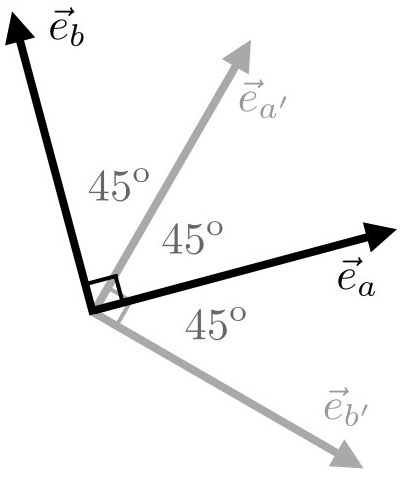
\includegraphics[width=1.5in]{vectorsCHSH.jpeg}
 \caption{Measurement directions for maximum violation of the CHSH inequality.}
   \label{vectorsCHSH}
\end{figure}

To reach the Tsirelson bound we need both of the expectation values in Eqs.\ (\ref{CHSH-Tsirelson 1})--(\ref{CHSH-Tsirelson 2}) to vanish. This occurs when the unit vectors for the measurement settings of Alice and Bob are related as 
\begin{equation}
\vec{e}_{a'}=\frac{1}{\sqrt{2}}\vec{e}_a+\frac{1}{\sqrt{2}}\vec{e}_b,\quad \vec{e}_{b'}= \frac{1}{\sqrt{2}}\vec{e}_a- \frac{1}{\sqrt{2}}\vec{e}_b. 
\end{equation}
Squaring the first of these relations, we find that
\begin{equation}
1 = \left( \vec{e}_{a'} \right)^2 = \left( \frac{1}{\sqrt{2}}\vec{e}_a+\frac{1}{\sqrt{2}}\vec{e}_b \right)^2 = \frac12 + \frac12 + \vec{e}_{a} \! \cdot \vec{e}_{b},
\end{equation}
from which it follows that $\vec{e}_{a} \perp \vec{e}_{b}$. The situation is thus as shown in Figure \ref{vectorsCHSH}. It follows that $\varphi_{ab} =  \varphi_{a'b'} = 90^{\mathrm{o}}$, $\varphi_{aa'} =  \varphi_{ab'} = \varphi_{ba'} = 45^{\mathrm{o}}$ and $\varphi_{bb'} =  135^{\mathrm{o}}$. Hence
\begin{equation*}
\chi_{ab}=\chi_{a'b'}= \cos{90^{\mathrm{o}}} = 0,
\end{equation*}
\begin{equation}
\chi_{aa'}=\chi_{ba'}=\chi_{ab'}= \cos{45^{\mathrm{o}}} = \frac{1}{\sqrt{2}},
\end{equation}
\begin{equation*}
\chi_{bb'}= \cos{135^{\mathrm{o}}} = - \frac{1}{\sqrt{2}}.
\end{equation*}
In this case we therefore have
\begin{equation}
\chi_{aa'}+\chi_{ab'}+\chi_{ab'}-\chi_{bb'} =2\sqrt{2}.
\label{CHSH-Tsirelson 5}
\end{equation}
This represents the maximum violation of the CHSH inequality and we see once again that the set of quantum correlations is larger than the local polytope.

As was noted in Section \ref{1.4} for the three-settting case, however, Tsirelson's bound is a necessary but not sufficient condition for quantum correlations. To see this presently, note that \emph{every} possible expectation value of the form Eqs. (\ref{CHSH-Tsirelson 1})--(\ref{CHSH-Tsirelson 2}) ought to be non-negative. But each such expectation gives rise to another linear inequality on the six anti-correlation coefficients. For instance, if Bob were to instead use $(-\hat{a}',-\hat{b}')$ then the inequality obtained is 
\begin{equation}
\chi_{aa'}+\chi_{ab'}+\chi_{ab'}-\chi_{bb'}\geq -2\sqrt{2}.
\label{CHSH-Tsirelson 6}
\end{equation}
The anti-correlation coefficients therefore satisfy not one but infinitely many linear bounds, all of which must be satisfied if the coefficients arise quantum-mechanically. Hence Tsirelson's bound is evidently not sufficient to characterize the set of quantum correlations in the CHSH setup and moreover no finite list of such inequalities will suffice either. The set of quantum correlations in the CHSH setup is therefore not a polytope and is instead some smooth convex body.

As was the case for the 3-elliptope in relation to the three-setting case, however, this still leaves the possibility to characterize the set of quantum correlations by \emph{nonlinear} inequalities. To find these it is useful to relate the set of quantum correlations for the four-setting case to those for the three-setting case. For instance, suppose Alice and Bob are allowed to use three of the four settings, e.g., Alice and Bob measure using settings $(\hat{a},\hat{b},\hat{a}')$. The results of Section \ref{1.5} then apply and therefore the anti-correlation coefficients $(\chi_{ab},\chi_{aa'},\chi_{ba'})$ must lie within the corresponding 3-elliptope:
\begin{equation}
1-\chi_{ab}^2-\chi_{aa'}^2-\chi_{ba'}^2+2\chi_{ab}\chi_{aa'}\chi_{ba'}\geq 0.
\label{3-elliptope}
\end{equation}
In mathematical terms, this is an application of Sylvester's criterion: A matrix is positive semi-definite if and only if none of its principal minors are negative. It is then useful to rewrite the 3-elliptope in the equivalent form\footnote{Aside from an overall square root, this form of the inequality (for three rather than four random variables) can be found in \citet[p.\ 486]{Yule 1896}. Cf.\ Eq.\ (\ref{lastminute}) in Section \ref{1.6}.}
\begin{equation}
 |\chi_{aa'}\chi_{ba'}-\chi_{ab}| \leq \sqrt{1-\chi_{aa'}^2}\sqrt{1-\chi_{ba'}^2}.
\end{equation}
The coefficient $\chi_{ab}$ cannot be deduced from Alice and Bob's measurements in the CHSH setup. Nevertheless this quantity does exist and the last inequality signifies that it cannot differ too much from $\chi_{aa'}\chi_{ba'}$. 
A similar calculation shows that, if Alice and Bob instead only made measurements on the settings $(\hat{a},\hat{b},\hat{b}'),$ then
\begin{equation}
 |\chi_{ab'}\chi_{bb'}-\chi_{ab}| \leq \sqrt{1-\chi_{ab'}^2}\sqrt{1-\chi_{bb'}^2}.
\end{equation}
We thus have bounds on how much $\chi_{ab}$ can differ from the values of $\chi_{aa'}\chi_{ba'}$ and $\chi_{ab'}\chi_{bb'}$. The triangle inequality then bounds how much these two quantities can differ from each other:
\begin{eqnarray}
|\chi_{aa'}\chi_{ba'}-\chi_{ab'}\chi_{bb'}|
&=& |(\chi_{aa'}\chi_{ba'}-\chi_{ab})+(\chi_{ab}-\chi_{ab'}\chi_{bb'})| \nonumber \\[.2cm]
&\leq & |\chi_{aa'}\chi_{ba'}-\chi_{ab}|+|\chi_{aa'}\chi_{ba'}-\chi_{ab}| \nonumber \\[.2cm]
&\leq & \sqrt{1-\chi_{aa'}^2}\sqrt{1-\chi_{ba'}^2}+\sqrt{1-\chi_{ab'}^2}\sqrt{1-\chi_{bb'}^2}.
\end{eqnarray}
Any set of anti-correlation coefficients obtained from measurements on the singlet state in the CHSH setup must satisfy this inequality, first obtained by \citet{Landau 1988}. The 3-elliptope therefore proves useful even when characterizing quantum correlations in the non-visualizable case of four settings.\footnote{It should be noted that we have only established that this this is a necessary condition for quantum correlations, i.e., if $\chi_{aa'}$, $\chi_{ab'}$, $\chi_{ba'}$ and $\chi_{bb'}$ do not satisfy Landau's inequality then one cannot find $\chi_{ab},\chi_{a'b'}$ such that $\chi$ is positive semi-definite (and therefore these are not quantum correlations). The converse claim, i.e., that Landau's inequality  is also a sufficient condition for quantum correlations, is beyond the scope of this paper and will not be addressed further.}

As an application of these results we consider again the special case where Alice and Bob share one setting, e.g. $\hat{b}'=\hat{b}$. Then $\chi_{bb'}=1$ and $\chi_{ab'}=\chi_{ab}$, so the second 3-elliptope inequality is then fulfilled trivially (both sides vanish identically) and Landau's result collapses to the 3-elliptope inequality. If we further relabel Bob's setting $\hat{a}'\to\hat{c}$, then this 3-elliptope takes the form
\begin{equation}
 |\chi_{ac}\chi_{bc}-\chi_{ab}| \leq \sqrt{1-\chi_{ac}^2}\sqrt{1-\chi_{bc}^2}.
\end{equation}
But this is the same 3-elliptope as considered originally in the Mermin example. Geometrically this means that the shadow of the 4-elliptope contains a copy of the 3-elliptope, occurring on the $\chi_{bb'}=1$ facet of the non-signaling hypercube.  This is as it should be:  The scenario where Alice and Bob, respectively, use settings $(\hat{a},\hat{b})$ and $(\hat{b},\hat{c})$ is exactly the setup originally employed by \citet{Bell 1964}. Combining this with the corresponding results for the local polytope and the non-signaling hypercube, we conclude that we recover the Mermin setup of Section \ref{1.4}--\ref{1.5} (including the entirety of Figure \ref{elliptope}) is indeed recovered when $\hat{b}'=\hat{b}$.

To concretely illustrate how the non-signaling hypercube, the set of quantum correlations and the local polytope are related, we consider the family of anti-correlation coefficients given by 
\begin{equation}
\chi_{aa'}=\chi_{ab'}=\chi_{ba'}=-\chi_{bb'}=-t
\end{equation}
for $0\leq t\leq 1$. The case $t=0$, where all correlation coefficients vanish, can be simulated classically (and therefore quantum mechanically), for instance by a raffle with basket containing all ticket types in equal proportion. By contrast, the case $t=1$ corresponds to the PR box shown in Figure \ref{CA-PRbox} in Section \ref{1.2} and should not be realizable in quantum mechanics despite being non-signaling. (More precisely, it is one of the vertices of the non-signaling hypercube which is not also a vertex of the local polytope).

The questions are then for what range of $t$ can such correlation coefficients be simulated classically or quantum-mechanically. For the classical case we observe that 
\begin{equation}
|\chi_{aa'}+\chi_{ab'}+\chi_{ba'}-\chi_{bb'}| =2t.
\end{equation}
Since the CHSH inequality bounds this magnitude by $2$, we conclude that $t\leq 1/2$ is the classical bound. For the quantum case we appeal to Landau's inequality, which takes the form
\begin{eqnarray}
|\chi_{aa'}\chi_{ba'}-\chi_{ab'}\chi_{bb'}| & \!\! = \!\! & 2t^2 \nonumber \\[.1cm]
& \!\!  \leq \!\! & \sqrt{1-\chi_{aa'}^2}\sqrt{1-\chi_{ba'}^2}+\sqrt{1-\chi_{ab'}^2}\sqrt{1-\chi_{bb'}^2}  \\[.2cm]
&  \!\! = \!\!  & 2(1-t^2). \nonumber
\end{eqnarray}
We therefore conclude that $t\leq 1/\sqrt{2}$, corresponding to Tsirelson's bound, i.e., the maximal violation of the CHSH inequality, marks the boundary between quantum and non-quantum correlations along this family of anti-correlation coefficients.% The relation between these cases is illustrated in [Figure].
